
%%%%%%%%%%%%%%%%%%%%%%%%%%%%%%%%%%%%%%%%%%%%%%%%%%%%%%%%%%%%%%%%%%%%%
%% This is a (brief) model paper using the achemso class
%% The document class accepts keyval options, which should include
%% the target journal and optionally the manuscript type.
%%%%%%%%%%%%%%%%%%%%%%%%%%%%%%%%%%%%%%%%%%%%%%%%%%%%%%%%%%%%%%%%%%%%%
\documentclass[journal=jacsat,manuscript=article]{achemso}

%%%%%%%%%%%%%%%%%%%%%%%%%%%%%%%%%%%%%%%%%%%%%%%%%%%%%%%%%%%%%%%%%%%%%
%% Place any additional packages needed here.  Only include packages
%% which are essential, to avoid problems later.
%%%%%%%%%%%%%%%%%%%%%%%%%%%%%%%%%%%%%%%%%%%%%%%%%%%%%%%%%%%%%%%%%%%%%
\usepackage[pdftex,dvipsnames]{xcolor}  % Coloured text etc.
\usepackage{xargs}                      % Use more than one optional parameter in a new commands
\usepackage{chemformula} % Formula subscripts using \ch{}
\usepackage[T1]{fontenc} % Use modern font encodings
\usepackage[utf8]{inputenc}
\usepackage{hyperref}
\usepackage{listings}
\usepackage[percent]{overpic}
\usepackage{subcaption}
\usepackage[export]{adjustbox}
\usepackage{longtable}
\usepackage{pdflscape}
\usepackage{graphicx}
%\usepackage[margin=0.25in]{geometry}
%\usepackage{pgfplots}
% 
\usepackage[colorinlistoftodos,prependcaption,textsize=tiny]{todonotes}
\newcommandx{\unsure}[2][1=]{\todo[linecolor=red,backgroundcolor=red!25,bordercolor=red,#1]{#2}}
\newcommandx{\change}[2][1=]{\todo[linecolor=blue,backgroundcolor=blue!25,bordercolor=blue,#1]{#2}}
\newcommandx{\info}[2][1=]{\todo[linecolor=OliveGreen,backgroundcolor=OliveGreen!25,bordercolor=OliveGreen,#1]{#2}}
\newcommandx{\improvement}[2][1=]{\todo[linecolor=Plum,backgroundcolor=Plum!25,bordercolor=Plum,#1]{#2}}
\newcommandx{\thiswillnotshow}[2][1=]{\todo[disable,#1]{#2}}

\lstdefinelanguage{viamd}
{
    morekeywords=[1]{=, <=, >=, !=, ==, and, or, xor, not, of, in, out},
    morekeywords=[2]{import, all, name, type, label, atom, resname, element, residue, resid, chain, distance, distance_min, distance_max, distance_pair, angle, dihedral, within, within_x, within_y, within_z, within_xyz, protein, water, ion, ring, x, y, z, flatten, count, com, rdf, sdf, plane, rmsd},
    morekeywords=[3]{int, irange, float, frange, string, bitfield, void, position, volume, distribution}
    keywordstyle=[1]\color{magenta},
    keywordstyle=[2]\color{blue},
    keywordstyle=[3]\color{red},
    sensitive=true,
    morecomment=[l]{\#},
    morestring = [b]",
    morestring = [b]',
}

\definecolor{codegreen}{rgb}{0,0.6,0}
\definecolor{codegray}{rgb}{0.5,0.5,0.5}
\definecolor{codepurple}{rgb}{0.58,0,0.82}
\definecolor{backcolour}{rgb}{0.95,0.95,0.92}

\lstdefinestyle{viamdstyle}{
    backgroundcolor=\color{backcolour},   
    commentstyle=\color{codegreen},
    numberstyle=\tiny\color{codegray},
    stringstyle=\color{codepurple},
    keywordstyle=\color{magenta},
    basicstyle=\ttfamily\footnotesize,
    breakatwhitespace=false,         
    breaklines=true,                 
    captionpos=b,                    
    keepspaces=true,                 
    numbers=left,                    
    numbersep=5pt,                  
    showspaces=false,                
    showstringspaces=false,
    showtabs=false,                  
    tabsize=2
}

\lstset{style=viamdstyle}

% Variables for indexing the different views in the overview
%\def \view:spatial {a}
%\def \view:representation {b}
%\def \view:animation{c}
%\def \view:script {d}
%\def \view:ramachandran {e}
%def \view:temporal {f}
%\def \view:volume {g}
%\def \view:distribution {h}
%\def \view:shape_space {i}

%%%%%%%%%%%%%%%%%%%%%%%%%%%%%%%%%%%%%%%%%%%%%%%%%%%%%%%%%%%%%%%%%%%%%
%% If issues arise when submitting your manuscript, you may want to
%% un-comment the next line.  This provides information on the
%% version of every file you have used.
%%%%%%%%%%%%%%%%%%%%%%%%%%%%%%%%%%%%%%%%%%%%%%%%%%%%%%%%%%%%%%%%%%%%%
%%\listfiles

%%%%%%%%%%%%%%%%%%%%%%%%%%%%%%%%%%%%%%%%%%%%%%%%%%%%%%%%%%%%%%%%%%%%%
%% Place any additional macros here.  Please use \newcommand* where
%% possible, and avoid layout-changing macros (which are not used
%% when typesetting).
%%%%%%%%%%%%%%%%%%%%%%%%%%%%%%%%%%%%%%%%%%%%%%%%%%%%%%%%%%%%%%%%%%%%%
\newcommand*\new[1]{\textcolor{blue}{#1}}
\newcommand*\rotcell[1]{\rotatebox{60}{\strut #1}}

%%%%%%%%%%%%%%%%%%%%%%%%%%%%%%%%%%%%%%%%%%%%%%%%%%%%%%%%%%%%%%%%%%%%%
%% Meta-data block
%% ---------------
%% Each author should be given as a separate \author command.
%%
%% Corresponding authors should have an e-mail given after the author
%% name as an \email command. Phone and fax numbers can be given
%% using \phone and \fax, respectively; this information is optional.
%%
%% The affiliation of authors is given after the authors; each
%% \affiliation command applies to all preceding authors not already
%% assigned an affiliation.
%%
%% The affiliation takes an option argument for the short name.  This
%% will typically be something like "University of Somewhere".
%%
%% The \altaffiliation macro should be used for new address, etc.
%% On the other hand, \alsoaffiliation is used on a per author basis
%% when authors are associated with multiple institutions.
%%%%%%%%%%%%%%%%%%%%%%%%%%%%%%%%%%%%%%%%%%%%%%%%%%%%%%%%%%%%%%%%%%%%%
\author{Robin Skånberg}
\affiliation[PDC]{PDC Center for High Performance Computing, KTH Royal Institute of Technology, SE-100 44 Stockholm, Sweden}
\email{robsk@kth.se}

\author{Gustav Eriksson}
\affiliation[LIU]{Linköping University, SE-581 83 Linköping,
Sweden}

\author{Tobias Pettersson}
\affiliation[LIU]{Linköping University, SE-581 83 Linköping,
Sweden}

\author{Mohit Sharma}
\affiliation[LIU]{Linköping University, SE-581 83 Linköping,
Sweden}

\author{Iulia Brumboiu}
\affiliation[UMK]{Nicolaus Copernicus University (UMK), Torun, Poland}

\author{Josefine Hvarregaard Andersen}
\affiliation[UiT]{UiT The Arctic University of Norway}

\author{Xin Li}
\affiliation[PDC]{PDC Center for High Performance Computing, KTH Royal Institute of Technology, SE-100 44 Stockholm, Sweden}

\author{Talha Bin Masood}
\affiliation[LIU]{Linköping University, SE-581 83 Linköping,
Sweden}

\author{Patrick Norman}
\affiliation[PDC]{PDC Center for High Performance Computing, KTH Royal Institute of Technology, SE-100 44 Stockholm, Sweden}
\altaffiliation{Division of Theoretical Chemistry and Biology, School of Engineering Sciences in Chemistry,
Biotechnology and Health, KTH Royal Institute of
Technology, SE-100 44 Stockholm, Sweden}

\author{Mathieu Linares}
\affiliation[PDC]{PDC Center for High Performance Computing, KTH Royal Institute of Technology, SE-100 44 Stockholm, Sweden}
\email{linares@kth.se}

%%%%%%%%%%%%%%%%%%%%%%%%%%%%%%%%%%%%%%%%%%%%%%%%%%%%%%%%%%%%%%%%%%%%%
%% The document title should be given as usual. Some journals require
%% a running title from the author: this should be supplied as an
%% optional argument to \title.
%%%%%%%%%%%%%%%%%%%%%%%%%%%%%%%%%%%%%%%%%%%%%%%%%%%%%%%%%%%%%%%%%%%%%
\title{Interactive Quantum Chemical Analysis: VIAMD and VeloxChem 1.0 Integration}

%%%%%%%%%%%%%%%%%%%%%%%%%%%%%%%%%%%%%%%%%%%%%%%%%%%%%%%%%%%%%%%%%%%%%
%% Some journals require a list of abbreviations or keywords to be
%% supplied. These should be set up here, and will be printed after
%% the title and author information, if needed.
%%%%%%%%%%%%%%%%%%%%%%%%%%%%%%%%%%%%%%%%%%%%%%%%%%%%%%%%%%%%%%%%%%%%%
\abbreviations{VIAMD, HDF5, GTO, AO, MO, SCF, TDDFT, NTO, CPP, IR, PNA, RESP}
\keywords{Molecular visualization, Electronic structure, VeloxChem, HDF5, Molecular orbitals, TDDFT, Transition density, Interactive analysis}

%%%%%%%%%%%%%%%%%%%%%%%%%%%%%%%%%%%%%%%%%%%%%%%%%%%%%%%%%%%%%%%%%%%%%
%% The manuscript does not need to include \maketitle, which is
%% executed automatically.
%%%%%%%%%%%%%%%%%%%%%%%%%%%%%%%%%%%%%%%%%%%%%%%%%%%%%%%%%%%%%%%%%%%%%
\begin{document}

%%%%%%%%%%%%%%%%%%%%%%%%%%%%%%%%%%%%%%%%%%%%%%%%%%%%%%%%%%%%%%%%%%%%%
%% The "tocentry" environment can be used to create an entry for the
%% graphical table of contents. It is given here as some journals
%% require that it is printed as part of the abstract page. It will
%% be automatically moved as appropriate.
%%%%%%%%%%%%%%%%%%%%%%%%%%%%%%%%%%%%%%%%%%%%%%%%%%%%%%%%%%%%%%%%%%%%%
\begin{tocentry}
\centering
\includegraphics[scale=0.135]{figure/toc.png}
\end{tocentry}

%%%%%%%%%%%%%%%%%%%%%%%%%%%%%%%%%%%%%%%%%%%%%%%%%%%%%%%%%%%%%%%%%%%%%
%% The abstract environment will automatically gobble the contents
%% if an abstract is not used by the target journal.
%%%%%%%%%%%%%%%%%%%%%%%%%%%%%%%%%%%%%%%%%%%%%%%%%%%%%%%%%%%%%%%%%%%%%
\begin{abstract}
Quantum-chemical analysis often requires moving between electronic-structure programs, intermediate grid files, molecular viewers, and plotting tools. This fragmented workflow complicates the interactive interpretation of molecular orbitals, electron densities, spectra, response properties, and excited-state descriptors. We present the integration of VIAMD with VeloxChem 1.0, enabling direct loading and interactive analysis of VeloxChem HDF5 output files. The interface exposes calculation metadata, SCF and geometry-convergence information, molecular orbitals, total and difference densities, TDDFT spectra, IR spectra, vibrational modes, attachment and detachment densities, transition moments, fragment-based charge-transfer analysis, and density critical points within a single visualization environment. The implementation reconstructs Gaussian-type-orbital basis data from the VeloxChem output, evaluates volumetric electronic representations on demand, and reuses the same parsed data model across summary, response, orbital-grid, and transition-analysis views. First CPU benchmarks on representative VeloxChem datasets show millisecond-scale HDF5 parsing and interactive molecular-orbital volume generation for small and medium examples. The integration reduces reliance on precomputed cube files and provides a unified route from quantum-chemical output to visual interpretation.
\end{abstract}

%%%%%%%%%%%%%%%%%%%%%%%%%%%%%%%%%%%%%%%%%%%%%%%%%%%%%%%%%%%%%%%%%%%%%
%% Start the main part of the manuscript here.
%%%%%%%%%%%%%%%%%%%%%%%%%%%%%%%%%%%%%%%%%%%%%%%%%%%%%%%%%%%%%%%%%%%%%
\section{Introduction}

The visualization of results from electronic structure calculations is a cornerstone of quantum chemistry, helping researchers interpret molecular orbitals, electron densities, spectra, excited states, and related molecular properties. Traditional workflows often rely on standalone tools that interface with electronic structure programs to render orbital shapes and densities. Notable examples include Gaussian,~\cite{g16} which uses GaussView for orbital visualization, and programs such as ORCA,~\cite{ORCA} Q-Chem,~\cite{Q-Chem} and Turbomole,~\cite{Turbomole} which commonly generate grid-based files compatible with visualization tools such as VMD, PyMOL, Molden, Chimera, JSmol, Mol*, Avogadro, and dedicated wavefunction-analysis environments such as Multiwfn.~\cite{humphrey1996vmd,pymol,molden,pettersen2004ucsf,hanson2013jsmol,molstar,Hanwell2012Avogadro,Lu2012Multiwfn} Broader surveys of molecular visualization underline the maturity of structure-oriented rendering and analysis workflows, while also highlighting the continued need for domain-specific interactive tools that connect data, representation, and interpretation.~\cite{kozlikova2017visualization} Spectral data are often handled separately through scripts or external plotting utilities, enabling the study of absorption, emission, circular dichroism, and other spectroscopic properties.

Although these workflows are well established, their reliance on intermediate files and multiple specialized programs can lead to inefficient and fragmented analysis. Orbital visualization frequently depends on the generation of large grid files, such as cube files, whose size increases rapidly with system size, spatial resolution, and the number of orbitals or densities under investigation. Storing, transferring, and rendering these files can become cumbersome, especially when several electronic states or response properties are considered. Moreover, switching between separate tools for structure inspection, orbital visualization, spectral analysis, and excited-state interpretation makes it difficult to maintain an interactive connection between the molecular geometry and the underlying quantum chemical data.

VIAMD was originally developed as a C/C++ environment for visual interactive analysis of molecular dynamics data, with emphasis on the exploration of spatio-temporal molecular structures and derived properties.~\cite{VIAMD} Its interactive design makes it a natural platform for extending molecular visualization beyond classical trajectories toward quantum chemical analysis, where structure, electronic distributions, spectra, and state-specific properties should be inspected in a unified environment.

In this work, we present the integration of VIAMD with VeloxChem 1.0. VeloxChem is a Python-driven quantum chemistry program designed for high-performance simulations of molecular response properties at the Hartree--Fock, density-functional theory, and time-dependent density-functional theory levels.~\cite{Rinkevicius2020} It has been developed for efficient execution in high-performance computing environments, including recent GPU-accelerated implementations for demanding response calculations.~\cite{Velox-GPU} The integration described here provides native support in VIAMD for VeloxChem HDF5 output files, allowing molecular structures, orbitals, densities, spectra, and transition-analysis data to be loaded directly without conversion to external grid formats.

The aim of this article is to describe how this VIAMD--VeloxChem integration enables an interactive workflow for quantum chemical analysis. We focus on the direct loading of VeloxChem \texttt{.h5} files, the inspection of calculation metadata and convergence information, the visualization of molecular orbitals and electron densities, the analysis of electronic and vibrational spectra, and the interpretation of excited states through transition-analysis tools. The examples discussed throughout the article are based on VeloxChem input/output documentation datasets, which provide reproducible working cases for exploring the functionality described below.


\section{Initial Audit: Loading Data and the Summary Window}
VeloxChem HDF5 files can be opened from the \texttt{File > Load Data} menu or by dragging and dropping the file directly into the spatial view. After loading, VIAMD initializes the molecular structure and provides an immediate starting point for inspection, including a Ball and Stick representation and, when molecular orbital data are available, a default visualization of the highest occupied molecular orbital.

The Summary window, accessed through \texttt{Windows > VeloxChem > Summary}, provides the first audit of the loaded calculation. It reports the calculation level, including the method or functional and basis set, together with molecular metadata such as the number of atoms, charge, spin multiplicity, and number of electrons. The same window also exposes convergence information, including SCF convergence and, when present in the HDF5 file, geometry-convergence data for optimization-related calculations such as geometry optimizations, scan calculations, transition-state searches, and IRC paths.

The Summary window also contains interactive tables linked to the three-dimensional molecular view. Selecting an entry in the geometry table highlights the corresponding atom in the spatial view, allowing numerical coordinates and molecular structure to be inspected together. In addition, VIAMD computes critical point information from the electron density reconstructed from the molecular orbitals, following the long-established use of electron-density topology in quantum-chemical interpretation.\cite{Bader1990,Bader1991} The resulting critical point table is likewise interactive with the 3D view. This makes the Summary window a compact entry point for checking both the calculation metadata and the spatial features derived from the electronic density before moving to more specialized visualization and analysis tools.
\begin{figure}[!ht]
\centering
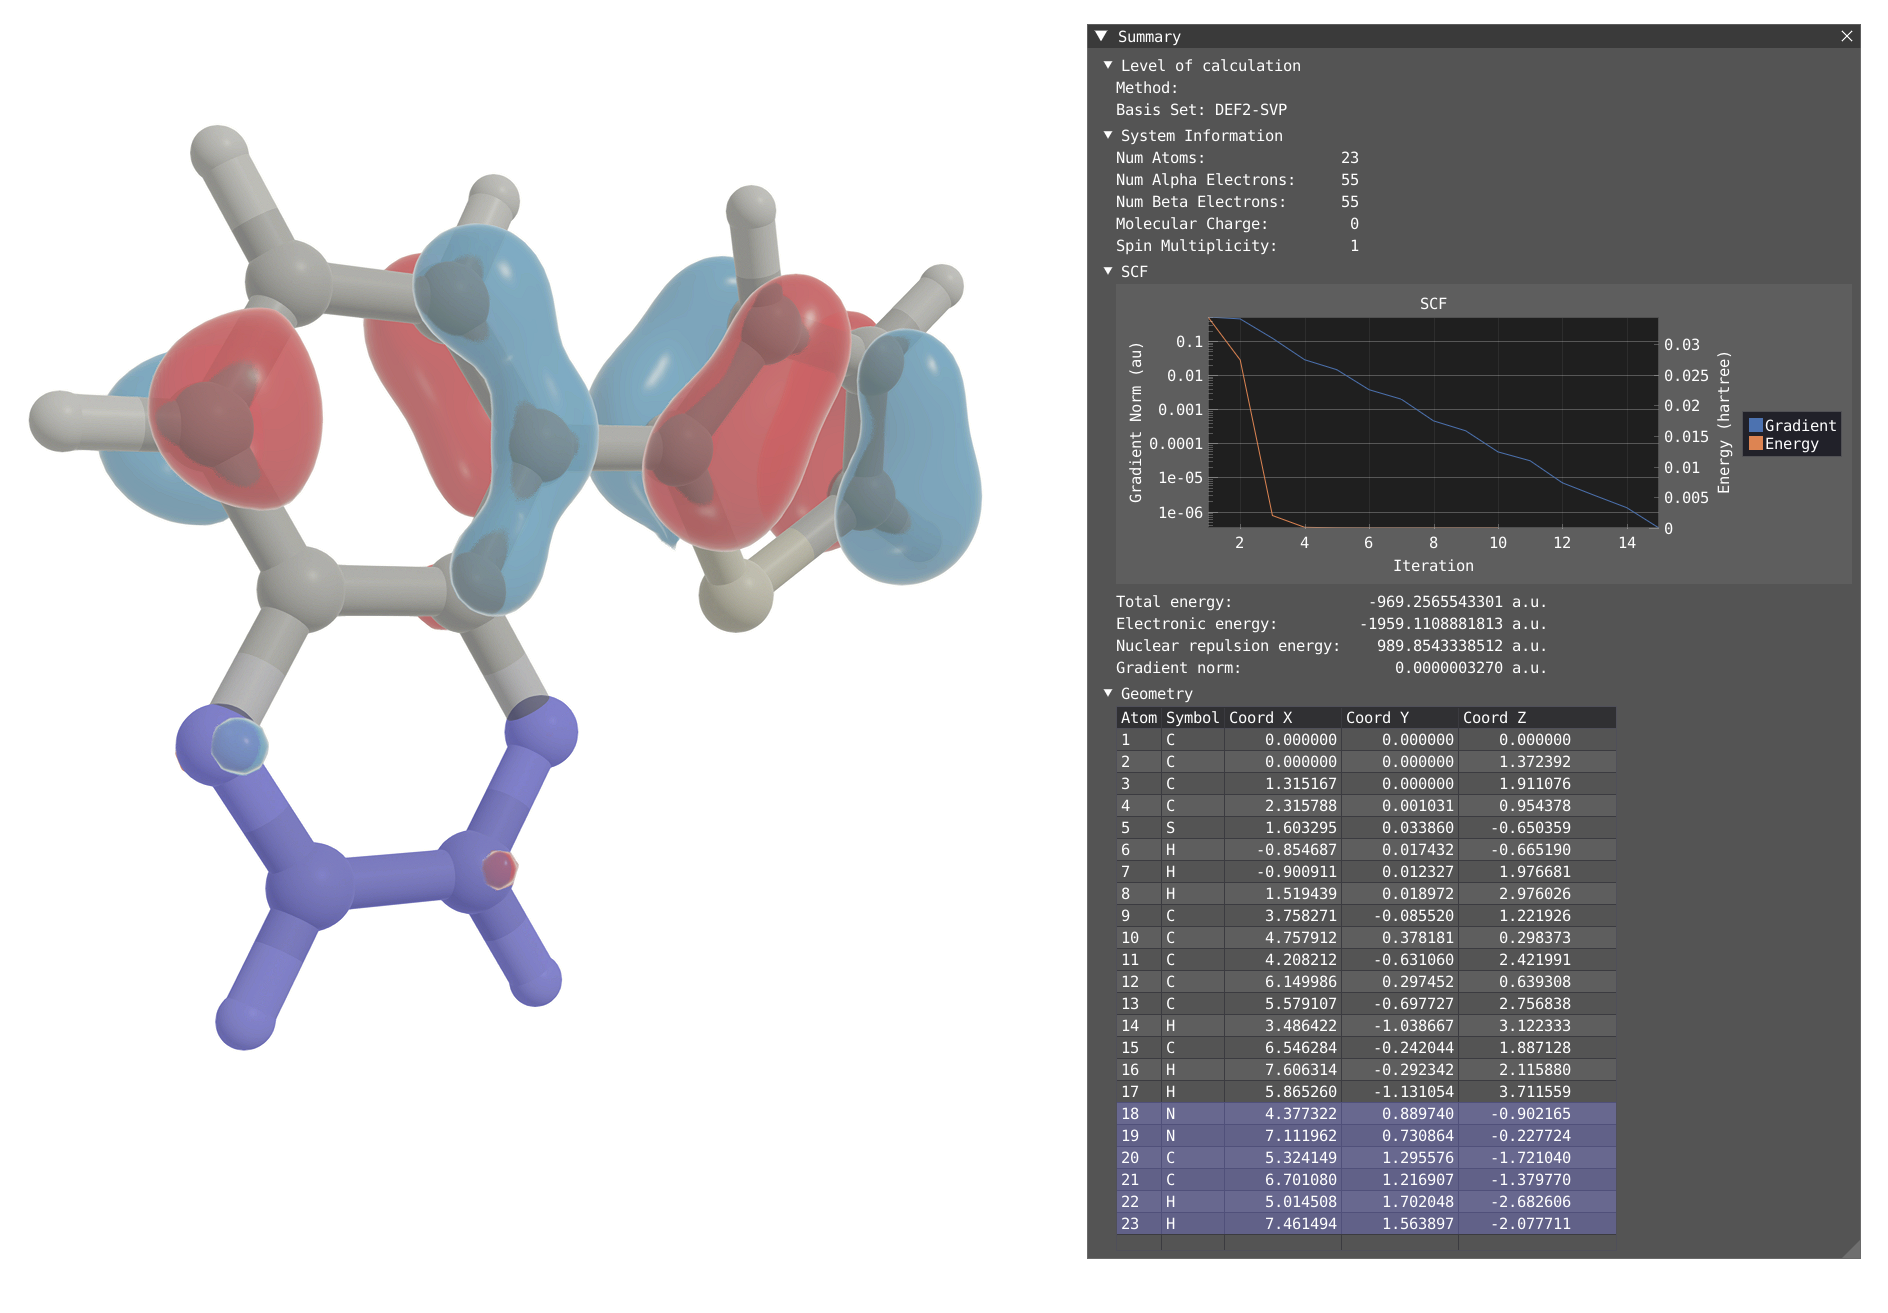
\includegraphics[width=0.9\textwidth]{figure/summary.png}
\caption{Summary window shown after loading a VeloxChem HDF5 dataset in VIAMD. The panel reports calculation metadata, SCF and geometry-convergence information when available, and interactive geometry and critical point tables linked to the three-dimensional molecular view.}
\label{fig:summary}
\end{figure}

\section{Visualizing the Electronic Landscape}
Electronic-structure data loaded from VeloxChem can be explored directly in the main VIAMD spatial view using the same representation workflow as for molecular structures. In addition to atomistic representations, users can add and configure volumetric electronic representations, choosing the underlying volume source according to the available data. These sources include molecular orbitals, orbital densities, total electron densities, Natural Transition Orbitals, attachment and detachment densities for TDDFT calculations, and density-related properties from complex polarization propagator calculations. The excited-state descriptors exposed here build on established analysis concepts such as Natural Transition Orbitals and attachment--detachment density analysis, which are widely used to reduce complex response data to chemically interpretable spatial patterns.\cite{Martin2003NTO,HeadGordon1995AttachDetach,Lu2012Multiwfn} VIAMD can also render differences between compatible volumetric sources, such as alpha--beta density differences, attachment--detachment density differences, or differences between selected NTO-related quantities. This makes it possible to inspect several electronic descriptors in the same interactive scene as the molecular geometry, while adjusting visual parameters such as isovalue, opacity, color, and phase convention.

The main spatial view can combine several kinds of quantum-chemical information in a single molecular scene. Four representative examples are used here to illustrate this range. The first is the HOMO representation created automatically when a VeloxChem file with molecular-orbital data is loaded, which provides an immediate electronic-structure starting point. The second combines a green total-electron-density isosurface with a molecular dipole or PNA representation, showing how volumetric scalar fields can be interpreted together with directional molecular descriptors. The third combines an electron-density isosurface with RESP-based atom coloring, linking the continuous density distribution to atom-centered electrostatic information derived from electrostatic-potential fitting or localized-property analysis.\cite{SinghKollman1984ESP,Bayly1993RESP,Gagliardi2004LoProp} The fourth uses an unrestricted calculation to display an alpha--beta density difference, making the spin imbalance visible as a signed volumetric representation. Together, these examples show that the representation system is not limited to isolated orbital plots, but can combine orbitals, densities, charge-derived coloring, vector or axis annotations, and spin-density differences within the same interactive view.

For comparative inspection, VIAMD also provides an Orbital Grid window, accessed through \texttt{Windows > VeloxChem > Orbital Grid}. The grid view is designed for rapid comparison of several orbitals or density-derived quantities side by side. Because this view contains many small electronic-structure panels together with energies, occupations, and selection controls, it is best presented as a large standalone figure rather than as one panel in the representation overview. Users can select the displayed orbital range, inspect energies and occupations, and compare changes in shape, phase, and localization across the electronic structure. The Orbital Grid also supports restricted open-shell and unrestricted calculations; for UHF data, alpha and beta orbital channels can be inspected separately. Together, the main-view representation controls and the Orbital Grid provide complementary workflows: detailed inspection of selected electronic features in the molecular scene and compact overview of multiple electronic states or orbitals.
\begin{figure}[!ht]
\centering
\begin{subfigure}[t]{0.48\textwidth}
\centering
\IfFileExists{figure/representation-homo.png}{%
\includegraphics[width=\textwidth]{figure/representation-homo.png}%
}{%
\fbox{\parbox[c][0.28\textwidth][c]{0.92\textwidth}{\centering Placeholder for HOMO representation loaded by default.}}%
}
\caption{Default HOMO representation generated when loading a VeloxChem dataset.}
\label{fig:representation-homo}
\end{subfigure}
\hfill
\begin{subfigure}[t]{0.48\textwidth}
\centering
\IfFileExists{figure/representation-density-dipole-pna.png}{%
\includegraphics[width=\textwidth]{figure/representation-density-dipole-pna.png}%
}{%
\fbox{\parbox[c][0.28\textwidth][c]{0.92\textwidth}{\centering Placeholder for green electron density with molecular dipole or PNA representation.}}%
}
\caption{Green total-electron-density isosurface shown together with a dipole or PNA representation.}
\label{fig:representation-density-dipole-pna}
\end{subfigure}

\begin{subfigure}[t]{0.48\textwidth}
\centering
\IfFileExists{figure/representation-density-resp.png}{%
\includegraphics[width=\textwidth]{figure/representation-density-resp.png}%
}{%
\fbox{\parbox[c][0.28\textwidth][c]{0.92\textwidth}{\centering Placeholder for electron density with RESP-colored molecular structure.}}%
}
\caption{Electron density combined with RESP-based atom coloring.}
\label{fig:representation-density-resp}
\end{subfigure}
\hfill
\begin{subfigure}[t]{0.48\textwidth}
\centering
\IfFileExists{figure/representation-alpha-beta.png}{%
\includegraphics[width=\textwidth]{figure/representation-alpha-beta.png}%
}{%
\fbox{\parbox[c][0.28\textwidth][c]{0.92\textwidth}{\centering Placeholder for alpha--beta density difference from a UHF calculation.}}%
}
\caption{Alpha--beta density difference for UHF data.}
\label{fig:representation-alpha-beta}
\end{subfigure}
\caption{Representative electronic-structure visualizations in VIAMD. The examples show the default HOMO generated upon loading a VeloxChem file, a green total-electron-density isosurface combined with a dipole or PNA representation, an electron-density representation with RESP-based atom coloring, and an alpha--beta density difference for an unrestricted calculation.}
\label{fig:electronic-landscape}
\end{figure}

\begin{figure}[!ht]
\centering
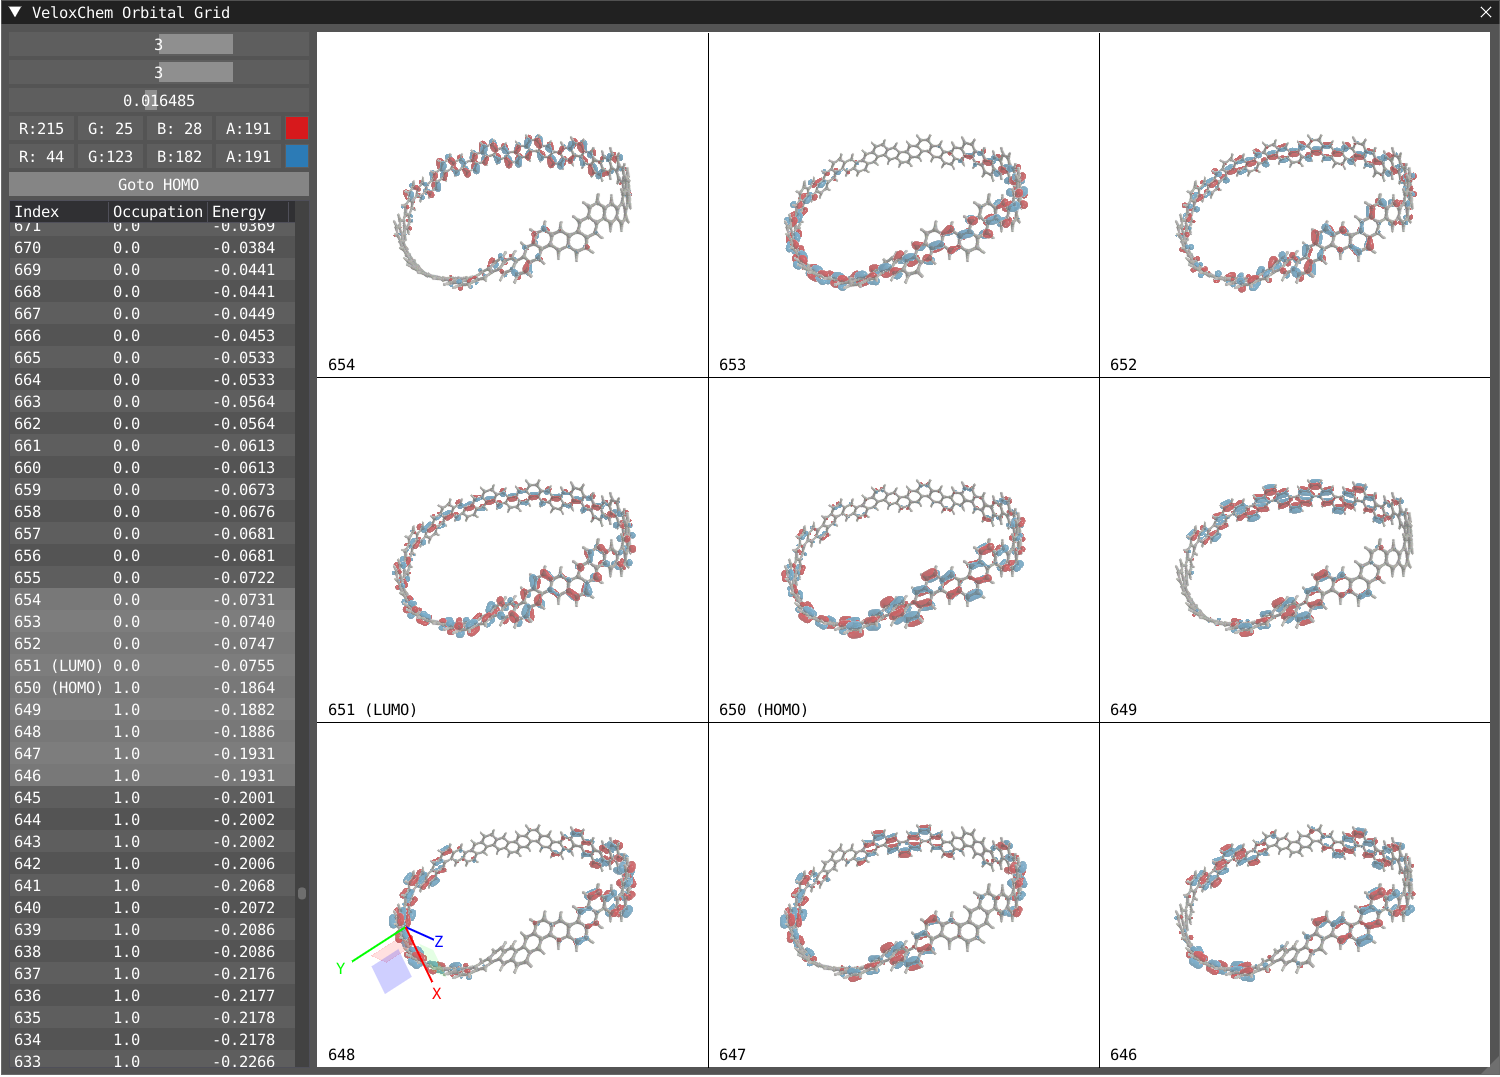
\includegraphics[width=\textwidth]{figure/orbital-grid.png}
\caption{Orbital Grid view for comparing multiple orbitals or density-derived quantities side by side. The window complements the main spatial representations by providing a compact overview of orbital shapes, phases, energies, occupations, and spin channels.}
\label{fig:orbital-grid}
\end{figure}

\section{Spectroscopy: Electronic and Vibrational Responses}
Spectroscopic observables provide a natural continuation of the electronic-structure visualization workflow. Once a VeloxChem HDF5 file has been loaded, VIAMD can expose response data through interactive spectral views and connect selected spectral features to molecular or electronic representations in the spatial view. In this article, we focus on two representative cases: TDDFT electronic spectroscopy and IR vibrational spectroscopy. TDDFT and response theory provide the underlying route from molecular electronic structure to excitation energies, oscillator strengths, optical activity, and related spectral observables.\cite{RungeGross1984,Casida1995,Rinkevicius2020} Other spectroscopic workflows supported by VeloxChem output, such as optical activity, CPP-based response calculations, Raman-type vibrational spectroscopy, and X-ray spectroscopies, follow the same general idea of linking spectral data to molecular interpretation, but are not discussed in detail here.

\subsection{Electronic spectroscopy from TDDFT}
The electronic-spectroscopy workflow is centered on the Response window, accessed through \texttt{Windows > VeloxChem > Response}. For TDDFT calculations, this window displays the discrete excited-state information as an interactive spectrum. The user can apply Lorentzian or Gaussian broadening, adjust the broadening width, and export the resulting spectral data to formats such as \texttt{.xvg} or \texttt{.csv}. This makes it possible to treat the spectrum not only as a final plot, but also as an interactive index into the excited states available in the calculation.

The connection between the spectral and spatial views is particularly useful for interpreting charge-transfer states. In the thiophene--quinoxaline example used here, the fourth excited state is selected from the TDDFT spectrum and visualized through the difference between attachment and detachment densities. This representation directly connects a peak in the electronic spectrum to the redistribution of electronic density during the excitation, and prepares the more detailed transition-analysis discussion in the next section.
\begin{figure}[!ht]
\centering
\IfFileExists{figure/tddft.png}{%
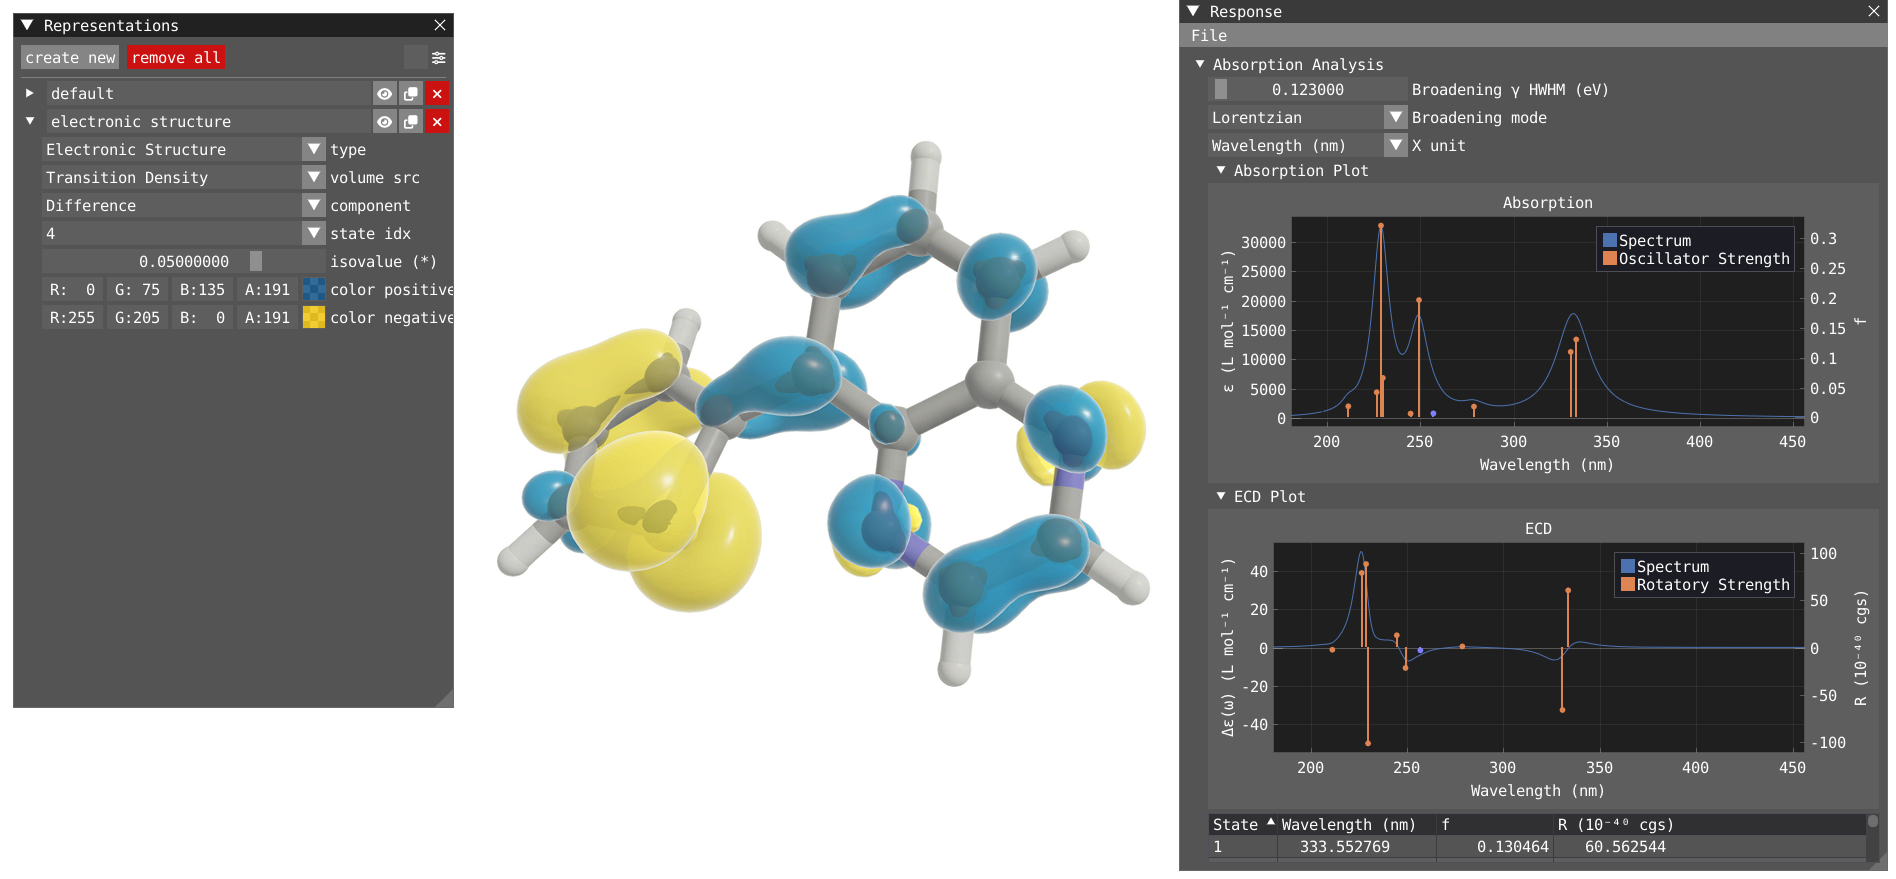
\includegraphics[width=0.9\textwidth]{figure/tddft.png}%
}{%
\fbox{\parbox[c][0.34\textwidth][c]{0.82\textwidth}{\centering Placeholder for TDDFT figure: interactive spectrum on the left and attachment--detachment density difference for the fourth TQ state on the right.}}%
}
\caption{TDDFT spectroscopy workflow in VIAMD. The interactive electronic spectrum is connected to a charge-transfer visualization for the fourth excited state of the TQ system, represented through the difference between attachment and detachment densities.}
\label{fig:tddft}
\end{figure}

\subsection{Vibrational spectroscopy from IR calculations}
For vibrational spectroscopy, VIAMD uses IR data as a representative workflow, also accessed through the Response window. Frequencies and intensities can be inspected as a vibrational spectrum, while individual peaks can be associated with the corresponding normal modes. Selecting a mode links the spectral information to the molecular geometry by animating the nuclear displacements directly in the three-dimensional view. This allows the user to move from a spectral feature to the underlying molecular motion without leaving the visualization environment.

\section{Advanced Transition Analysis: Charge Transfer and Transition Moments}
The transition-analysis tools in VIAMD follow the VALET approach for visual analysis of electronic densities and transitions in molecules.~\cite{MasoodCGF2021} After an excited state has been identified in the Response window, the corresponding electronic redistribution can be examined through attachment and detachment densities. These densities, together with NTOs and charge-transfer descriptors, form a standard toolbox for reducing many-orbital excited-state response data to chemically interpretable electron-removal, electron-attachment, and fragment-transfer patterns.\cite{HeadGordon1995AttachDetach,Martin2003NTO,LeBahers2011,Plasser2014} The detachment density indicates where electron density is removed during the excitation, while the attachment density indicates where electron density is accumulated. Their joint visualization, or their difference, provides a direct spatial description of the electronic rearrangement associated with the transition.

This workflow is complementary to the orbital and NTO visualizations described above, but the transition analysis itself is based on the attachment and detachment densities. In the TQ example, the charge-transfer character of the fourth excited state can therefore be inspected by comparing the regions of density depletion and accumulation in the molecular frame. The same view can be customized through settings controlling the attachment and detachment colors and the display of transition-related vectors.

In addition to density-based information, VIAMD can display the electric and magnetic transition dipole moment vectors for the selected state, together with the angle between them. Showing these vectors in the molecular frame helps relate the orientation of the transition moments to the molecular geometry and to the spatial pattern of the attachment and detachment densities.

For a more quantitative interpretation, users can define molecular subgroups or fragments and analyze how the attachment and detachment densities are distributed over them. This enables the characterization of local excitation versus charge-transfer character, for example by distinguishing density rearrangements localized on one molecular fragment from transitions involving donor--acceptor density displacement between different fragments.
\begin{figure}[!ht]
\centering
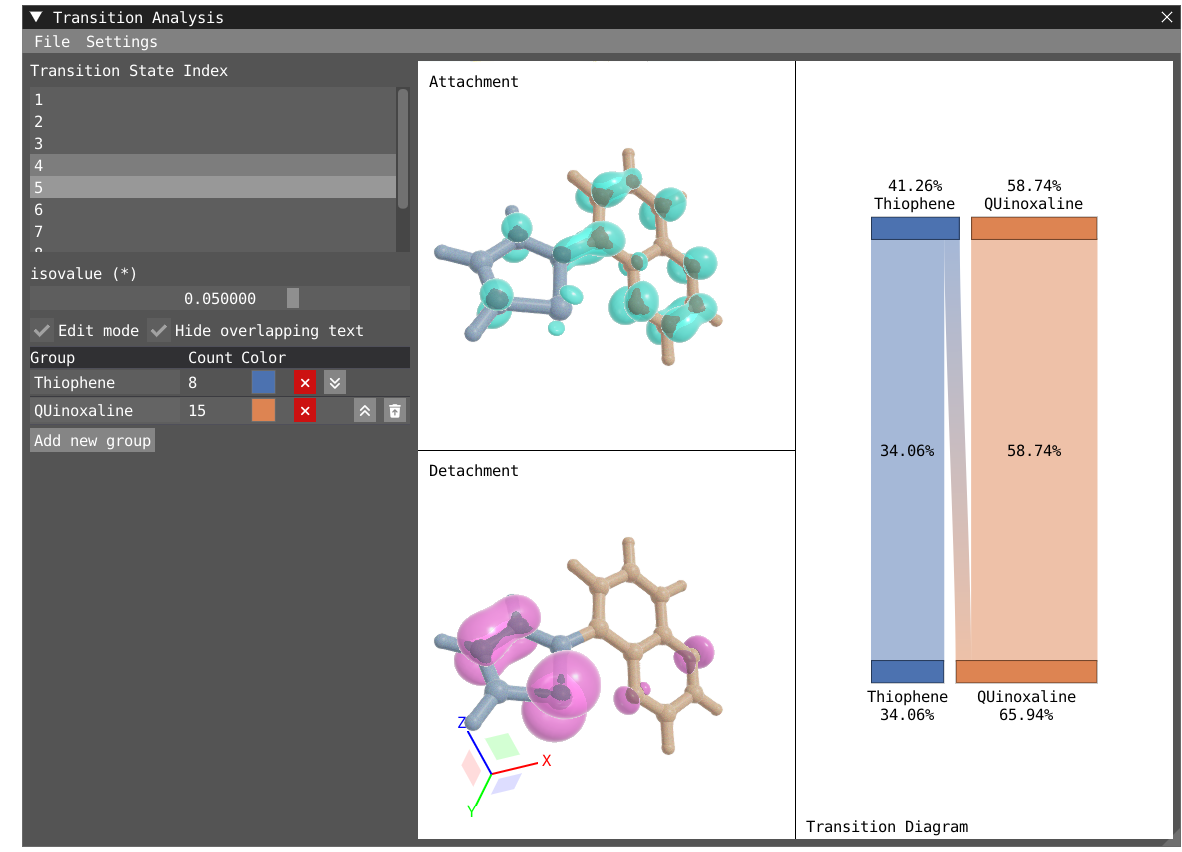
\includegraphics[width=0.9\textwidth]{figure/transition-analysis.png}
\caption{Transition-analysis workflow in VIAMD following the VALET approach. Attachment and detachment densities are used to analyze charge redistribution for a selected excited state, with customizable density colors, electric and magnetic transition dipole moment vectors, and the angle between them. Fragment definitions support quantification of local-excitation and charge-transfer character.}
\label{fig:transition-analysis}
\end{figure}

\section{Implementation}
The VeloxChem integration is implemented through the VIAMD loader system and the VeloxChem support layer in mdlib. When VeloxChem support is enabled, VIAMD registers HDF5 files with the \texttt{.h5} extension as VeloxChem datasets. HDF5 provides a portable hierarchical container for structured numerical data, which makes it well suited for storing molecular coordinates, basis information, orbital coefficients, response arrays, and derived properties in a single calculation file.\cite{HDF5} The generic loader initializes the molecular system from the file, while the VeloxChem component parses the complete quantum-chemical data into an \texttt{md\_vlx\_t} object. The parser reads the core molecular data and, when present, the \texttt{scf}, \texttt{rsp}, and \texttt{opt} HDF5 groups. These groups provide the data used throughout the interface: SCF orbital and density information, response data including excited-state and vibrational spectra, and optimization coordinates and energies. Atomic and density properties stored with the file are also exposed to the VIAMD property and representation systems.

A central step in the implementation is the conversion of VeloxChem basis and coefficient data into the Gaussian-type-orbital representation used by VIAMD. mdlib resolves the basis-set identifier, reads the corresponding basis description either from the packaged VIAMD basis resources or from the directory of the loaded file, normalizes the basis data, and builds an AO remapping table. The SCF coefficient and matrix data are then permuted into the canonical shell order expected by the GTO evaluator. The function that extracts the GTO basis produces an \texttt{md\_gto\_basis\_t}, while molecular-orbital coefficients and SCF density matrices are accessed directly from the parsed VeloxChem object. Restricted calculations share the same coefficient and density storage for the beta channel, whereas unrestricted calculations keep separate alpha and beta data; this is the basis for the alpha, beta, total, and difference choices exposed in the visualization interface.

Volumetric electronic representations are generated on demand rather than read from precomputed grid files. Each electronic representation stores its source, spin channel, orbital or excited-state index, transition-density component, NTO component, resolution, and frame-dependent state. VIAMD hashes these parameters and reevaluates the volume only when the hash changes. The sampling grid is constructed from the molecular bounds, and the resulting scalar field is stored in a three-dimensional OpenGL texture. Molecular orbitals and NTOs are evaluated from AO coefficient vectors over the GTO basis, whereas electron densities, transition densities, and density properties are evaluated from AO-space matrices. When the GPU path is available, coefficients, atom positions, and density matrices are packed into GPU buffers and evaluated with the mdlib GTO GPU routines before the result is uploaded to the rendering texture. Otherwise, VIAMD uses the OpenGL GTO grid-evaluation path.

The implementation of transition densities follows the data available in the VeloxChem response output. For a selected excited state, mdlib reads the TDDFT response solution vectors and constructs the transition quantity \(T = Z - Y\), using the de-excitation contribution when it is present. Attachment and detachment matrices are first formed in the virtual and occupied molecular-orbital spaces, respectively. These matrices are then transformed to the AO basis, symmetrized, and returned to VIAMD as attachment, detachment, or attachment--detachment difference matrices. VIAMD evaluates these matrices on the same GTO grid machinery as the ground-state density, which is why the main electronic representation system and the transition-analysis window use the same underlying volume-generation code.

The same parsed data model drives the other VeloxChem windows. The Summary window queries calculation labels, electron counts, charge, multiplicity, SCF history, optimization energies, and optimization coordinates from \texttt{md\_vlx\_t}. Critical-point analysis is computed inside VIAMD by evaluating an SCF density matrix on a grid and passing the resulting volume to the mdlib topology routines, after which the extracted graph is rendered and exposed through an interactive table. The Response window uses the response arrays for excitation energies, oscillator strengths, rotatory strengths, transition dipoles, CPP spectra, and vibrational IR data when those datasets are present. The Orbital Grid uses the same orbital coefficient accessors and GTO volume evaluation as the main representation system, but manages several small volumes simultaneously for side-by-side comparison. In this way, loading, summary inspection, orbital visualization, spectroscopy, and transition analysis all operate on one parsed VeloxChem HDF5 representation rather than on separate intermediate cube or plotting files.

\section{Performance}
The performance advantages of the VIAMD--VeloxChem workflow arise primarily from avoiding the repeated generation, storage, and loading of intermediate volumetric grid files. In a conventional cube-file workflow, each orbital, density, excited-state descriptor, or density difference must typically be exported as a separate grid file at a chosen spatial resolution. Exploring several orbitals, spin channels, excited states, or broadening choices can therefore produce many large files before the visualization step even begins. In VIAMD, the VeloxChem HDF5 file remains the central data source, and volumetric representations are reconstructed only when they are needed for visualization.

This design separates interactive visual changes from volumetric recomputation. Operations such as changing colors, opacity, isosurface signs, or the visibility of existing representations can be handled as rendering updates. More expensive operations, such as switching the orbital index, changing the spin channel, selecting a different excited state, changing the transition-density component, or increasing the volume resolution, trigger a new GTO-based volume evaluation. Because the representation state is hashed, VIAMD avoids unnecessary reevaluation when the underlying electronic-structure parameters have not changed.

The cost of a new volume evaluation depends on the number of atoms, the size of the AO basis, the selected representation type, the grid resolution, and the available hardware. Molecular orbitals and NTOs require evaluating one coefficient vector over the grid, whereas electron densities, density properties, and attachment or detachment densities require evaluating AO-space matrices. The latter are generally more demanding because the density evaluation involves pairwise basis-function contributions. Critical-point analysis adds another layer of cost because the electron density must first be evaluated on a grid and then processed by the topology routines. For this reason, the most expensive updates are those that combine high grid resolution with density-matrix evaluation and topological extraction.

When GPU support is available, VIAMD uses the mdlib GPU path to pack atom positions, coefficients, and density matrices into GPU buffers and evaluate the GTO volume on the compute device. The resulting scalar field is then transferred to an OpenGL texture for rendering. On systems where this path is not available, VIAMD relies on the OpenGL GTO grid-evaluation path. The user-facing behavior is the same in both cases: the expensive step is the generation of a new scalar field, while subsequent manipulation of the rendered representation remains interactive.

The direct HDF5 workflow also improves the practical performance of exploratory analysis in ways that are not captured by a single timing measurement. The user can move from molecular metadata to orbitals, spectra, vibrational modes, attachment and detachment densities, and transition moments without producing separate files for every intermediate question. This reduces disk usage, shortens the iteration cycle between calculation and interpretation, and keeps the molecular structure, spectra, and electronic descriptors synchronized inside one visualization session.

As a first benchmark, we measured representative CPU-side operations using the current Release build of VIAMD with VeloxChem/HDF5 support enabled, AVX/AVX2/FMA enabled, and the mdlib GPU path disabled. Each operation was repeated nine times and the median wall time was reported for a $64^3$ grid. For the small water dataset, HDF5 parsing took 1.3 ms and molecular-orbital volume generation took 3.9 ms. For the 26-atom molecule with 229 AOs, parsing took 3.2 ms and molecular-orbital volume generation took 31.7 ms. The TQ SCF dataset, with 23 atoms and 254 AOs, required 3.7 ms for parsing and 35.9 ms for molecular-orbital volume generation. For the acrolein response dataset, with 8 atoms, 76 AOs, and five excited states, parsing took 2.4 ms, molecular-orbital volume generation took 20.9 ms, and transition-density matrix extraction took 2.9 ms. These measurements should be interpreted as a first CPU baseline for the operations used by the visualization workflow; larger systems and GPU-enabled measurements will be added as additional datasets become available.

\begin{figure}[!ht]
\centering
\IfFileExists{figure/performance-timings.png}{%
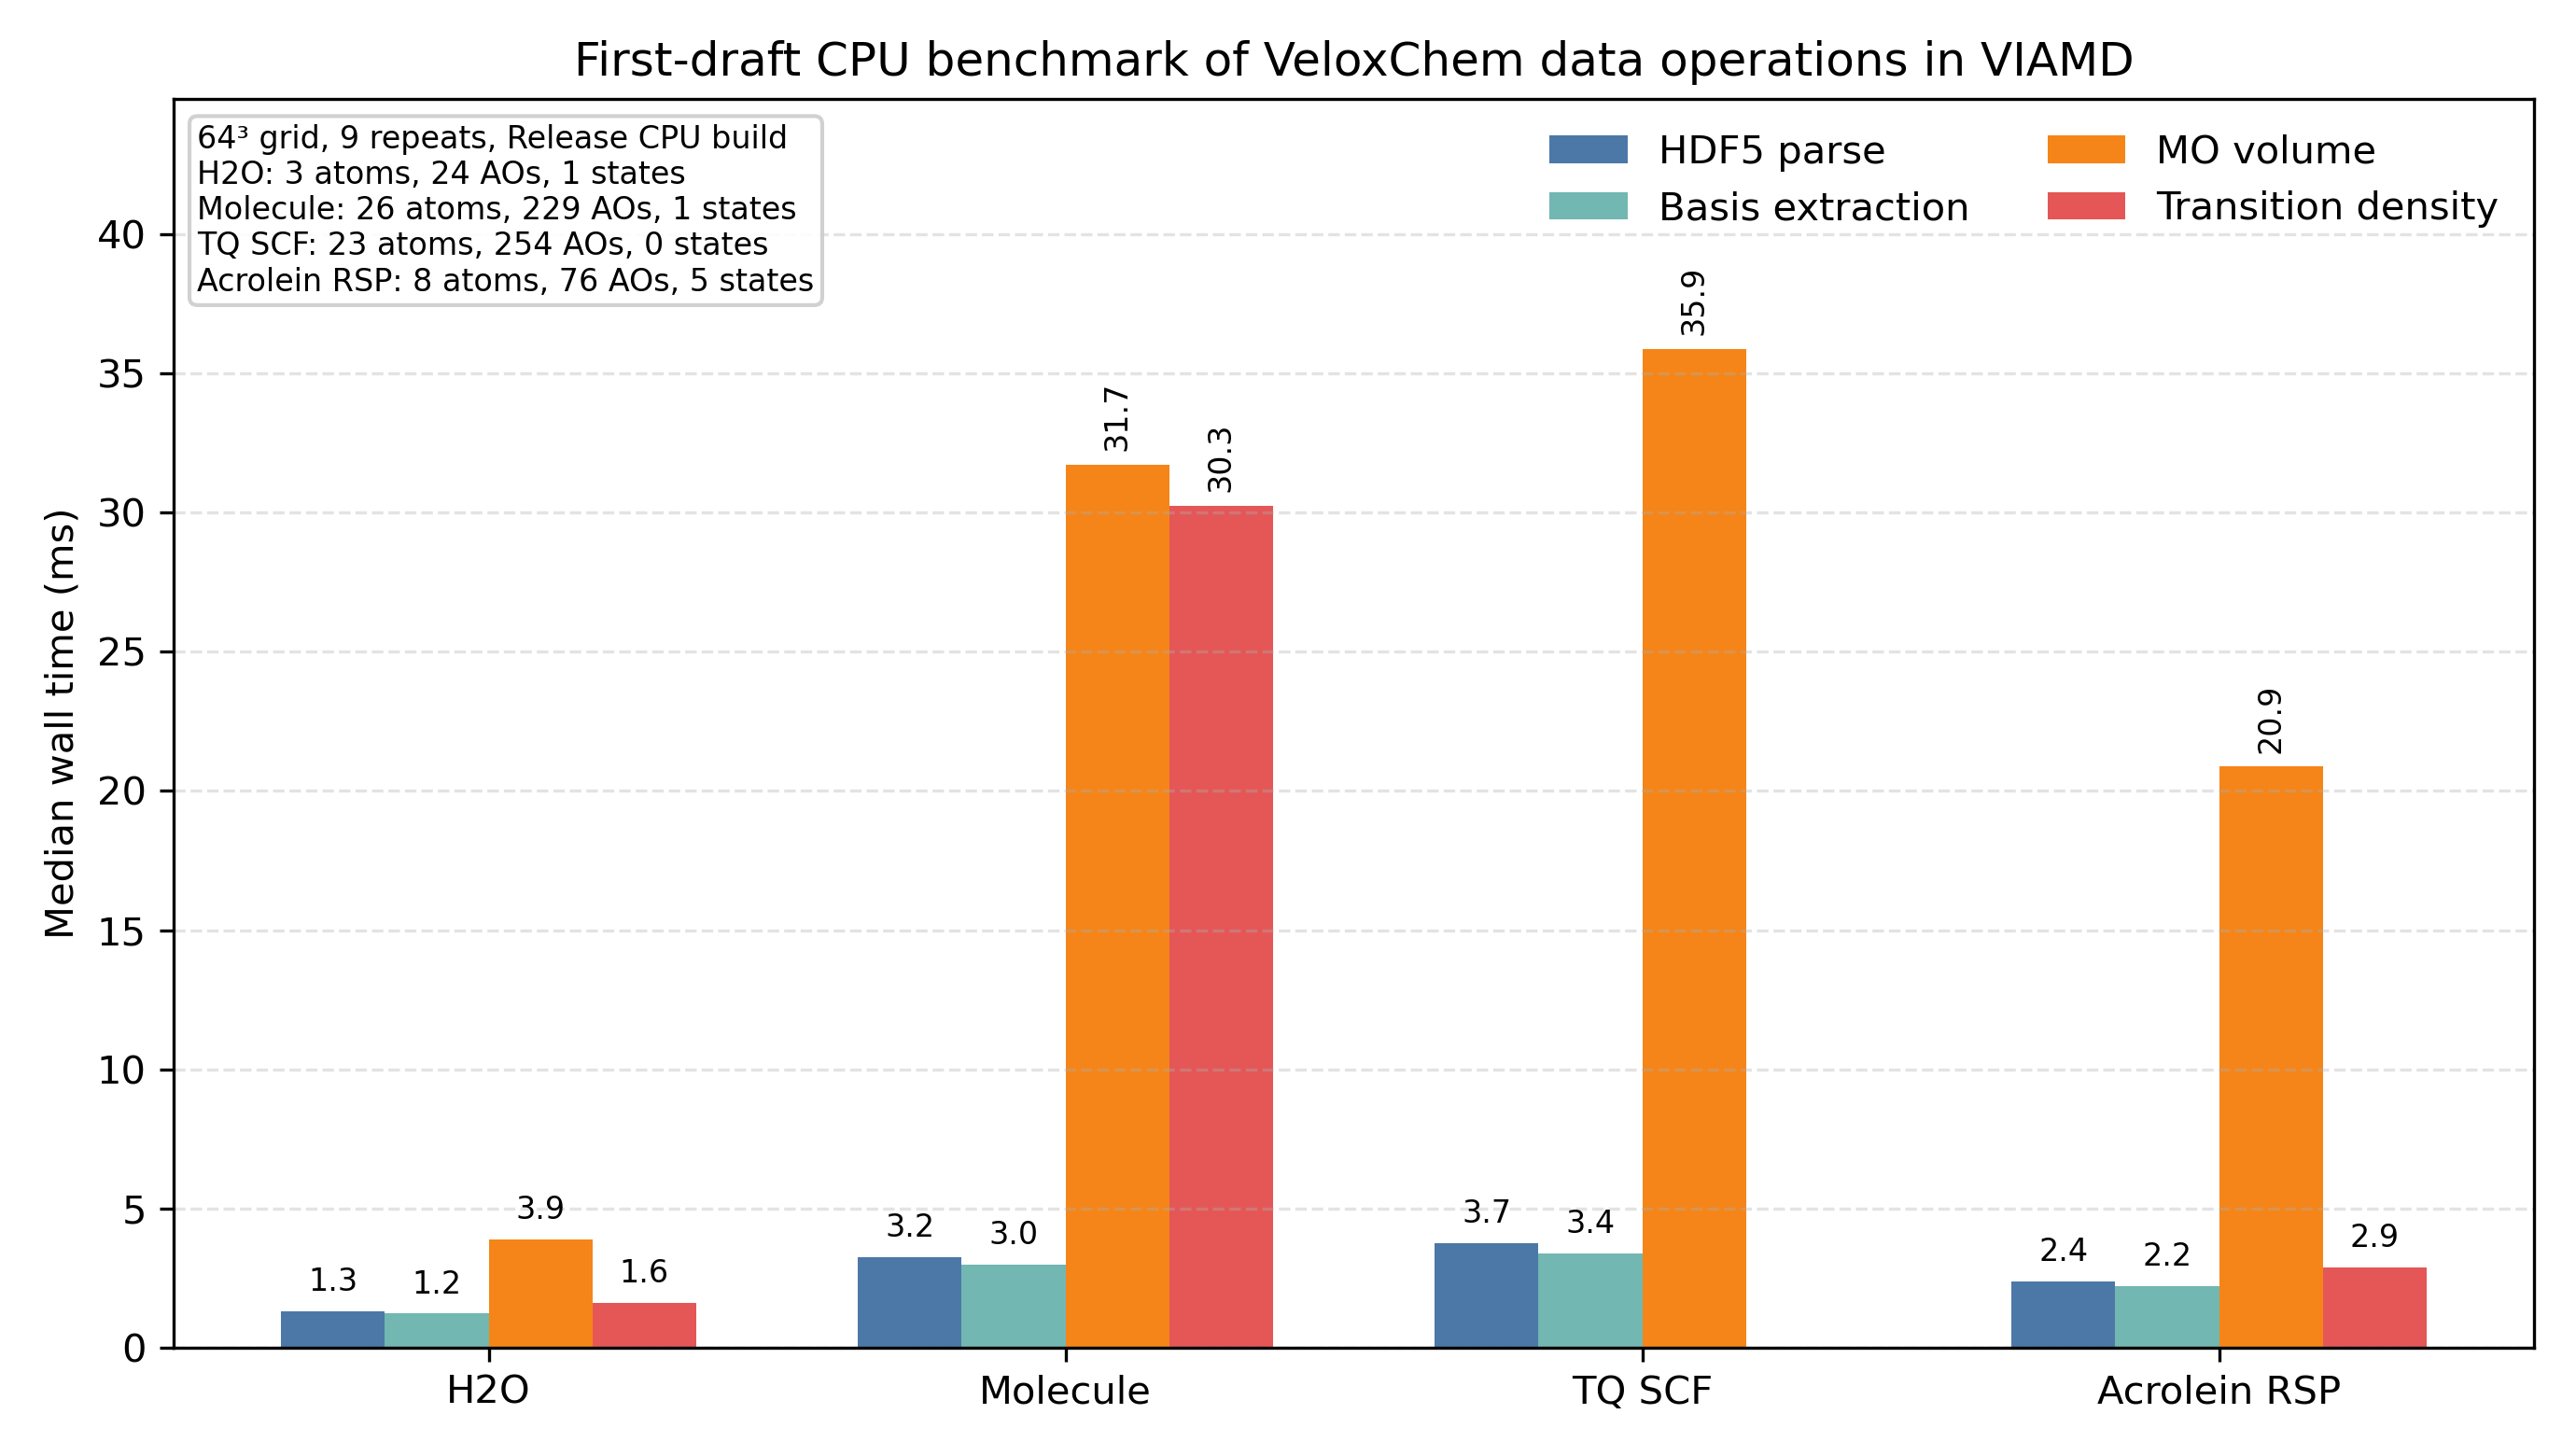
\includegraphics[width=0.9\textwidth]{figure/performance-timings.png}%
}{%
\fbox{\parbox[c][0.28\textwidth][c]{0.82\textwidth}{\centering Placeholder for performance timing figure: measured timings for HDF5 loading, orbital volumes, electron-density volumes, transition-density volumes, and critical-point extraction.}}%
}
\caption{First-draft CPU benchmark for representative VeloxChem workflows in VIAMD. Median wall times are reported for a $64^3$ grid over nine repeats using the current Release build with VeloxChem/HDF5 enabled and the mdlib GPU path disabled. Missing transition-density bars correspond to datasets without response-state data.}
\label{fig:performance-timings}
\end{figure}

\section{Workspace Management}
Interactive quantum-chemical analysis often involves more than a single visualization choice. A user may load a VeloxChem dataset, define several molecular and electronic representations, adjust isovalues and colors, select excited states or vibrational modes, define molecular fragments, and arrange camera views for comparison. VIAMD workspaces provide a way to preserve this analysis state in a \texttt{.via} file.

For VeloxChem datasets, a workspace can store the visual state of the molecular scene together with representation settings and custom subgroup definitions. This makes it possible to reopen the same HDF5 dataset and restore the analysis context without repeating all manual configuration steps. Workspaces are therefore useful both for continuing an exploratory session and for sharing a reproducible view of a specific orbital, density, transition, spectrum, or fragment analysis.

This capability complements the direct HDF5 workflow described above. The HDF5 file remains the source of the quantum-chemical data, while the workspace records how those data are inspected in VIAMD. Together, the calculation file and workspace file define a compact and reproducible analysis package.

\section{Conclusions}
We have presented the integration of VIAMD with VeloxChem 1.0 for interactive quantum-chemical analysis. By loading VeloxChem HDF5 output directly, VIAMD connects molecular structure, calculation metadata, convergence information, orbitals, densities, spectra, vibrational modes, transition densities, transition moments, and density critical points within a single visualization environment. This reduces the need for intermediate cube files and external plotting workflows while keeping the molecular and electronic data synchronized during analysis.

The implementation builds on a shared parsed VeloxChem data model, GTO-basis reconstruction, AO remapping, on-demand volume generation, and common access paths for the Summary, Response, Orbital Grid, and transition-analysis interfaces. First CPU benchmarks show that HDF5 parsing and molecular-orbital volume generation are fast for the representative datasets considered here, supporting interactive inspection on standard hardware. Future work will extend the benchmark set to larger molecular systems, include GPU-enabled measurements, and broaden the set of documented VeloxChem response and property workflows available through VIAMD.

\section{Author Contributions}
Robin Skånberg was the main developer of the code and contributed to the code design. Gustav Eriksson implemented the electronic-structure graphical interface, including interactive spectra, vibrational analysis, and transition analysis. Tobias Pettersson contributed to the transition-analysis functionality. Mohit Sharma provided the first implementation and guidelines for the critical point analysis. Iulia Brumboiu, Josefine Hvarregaard Andersen, and Xin Li contributed to the VeloxChem interface and provided user feedback on the graphical interface. Talha Bin Masood advised on electronic-structure computation, visualization, and topological analysis. Patrick Norman initiated the project, co-led the project, and contributed to the VeloxChem interface. Mathieu Linares led the project and contributed to the code design.

\begin{acknowledgement}

%Please use ``The authors thank \ldots'' rather than ``The authors would like to thank \ldots''.
The authors thank the Swedish e-Science Research Center (SeRC) and InfraVis.

\end{acknowledgement}

\section{Availability and Documentation}
The source code is freely available on \href{https://github.com/scanberg/viamd}{https://github.com/scanberg/viamd} under MIT license.
Precompiled VIAMD binaries are provided for Windows and macOS on both Intel and Apple Silicon architectures, while Linux build instructions are available through the VIAMD documentation.
VIAMD is under active development; therefore, design and implementation aspects may be subject to change. Documentation is available on the wiki page of VIAMD \href{https://github.com/scanberg/viamd/wiki}{https://github.com/scanberg/viamd/wiki} with pages dedicated to the software's visual, analysis, and language components. A series of tutorials is also proposed to encourage users to use VIAMD. In addition to VeloxChem HDF5 files, VIAMD supports TREXIO,~\cite{Trexio} a universal file format designed for interoperability across quantum chemistry software.

\subsection{Datasets}
The examples used in this article are based on the VeloxChem input/output file collection available from the VeloxChem documentation at \href{https://veloxchem.org/docs/input-files/}{https://veloxchem.org/docs/input-files/}. This collection provides paired input scripts, text input files, log files, and HDF5 output files for representative VeloxChem calculations. The HDF5 files are regenerated regularly from the VeloxChem master branch, and the VIAMD developers use this collection as a practical test set for checking the VeloxChem interface and the visualization features described in this article.

Table~\ref{tab:veloxchem-datasets} follows the organization of the VeloxChem input/output page and summarizes the VIAMD windows and feature families associated with each example. In the table, the Common column denotes the shared VIAMD starting point for VeloxChem HDF5 files: direct file loading; molecular-structure inspection; atom selection and highlighting through interactive tables; calculation metadata and convergence review in the Summary window; standard molecular representations in the spatial view; molecular-orbital, density, and density-difference representations when the required electronic-structure data are present; Orbital Grid comparison when orbital data are present; molecular vectors or axes when available; density topology and critical-point inspection when the density can be reconstructed; and saving or restoring the analysis state through VIAMD workspaces. The remaining columns mark additional interactive workflows available for specific examples. Vibrational spectra are included under the same Response workflow as electronic and other response-property spectra. The final column is restricted to atom-centered property datasets, such as ESP, RESP, Boltzmann-weighted RESP, and LoProp quantities.\cite{SinghKollman1984ESP,Bayly1993RESP,Gagliardi2004LoProp}

\begin{landscape}
{\footnotesize
\begin{longtable}{p{0.25\linewidth}p{0.25\linewidth}ccccc}
\caption{Draft feature matrix for VeloxChem input/output HDF5 files used to test and illustrate the VIAMD VeloxChem interface. The entries follow the order of the VeloxChem input/output documentation page. A bullet in the Common column denotes the shared VIAMD starting point: HDF5 loading, Summary-window metadata, molecular/electronic representations, Orbital Grid access when orbital data are present, molecular vectors or axes when present, density topology when density data allow it, and workspace saving. Optimisation marks geometry optimization, constrained-coordinate, scan, transition-state, and IRC workflows. Response covers electronic, vibrational, CPP, X-ray, and multiphoton response workflows. Transition marks attachment/detachment and charge-transfer analysis. Atomic props. marks atom-centered property datasets such as ESP, RESP, Boltzmann-weighted RESP, and LoProp. Feature availability should be verified against the monthly regenerated HDF5 files before final publication.}
\label{tab:veloxchem-datasets}\\
\hline
Example & HDF5 file & \rotcell{Common} & \rotcell{Optimisation} & \rotcell{Response} & \rotcell{Transition} & \rotcell{Atomic props.} \\
\hline
\endfirsthead
\hline
Example & HDF5 file & \rotcell{Common} & \rotcell{Optimisation} & \rotcell{Response} & \rotcell{Transition} & \rotcell{Atomic props.} \\
\hline
\endhead
SCF optimization & \texttt{biphenyl-scf.h5} & \(\bullet\) & -- & -- & -- & -- \\
ROHF optimization & \texttt{tempo-roscf.h5} & \(\bullet\) & -- & -- & -- & -- \\
UHF optimization & \texttt{trityl-uscf.h5} & \(\bullet\) & -- & -- & -- & -- \\
Static electric field & \texttt{pna-field.h5} & \(\bullet\) & -- & -- & -- & -- \\
CPCM environment & \texttt{eth-cpcm.h5} & \(\bullet\) & -- & -- & -- & -- \\
SMD environment & \texttt{eth-smd.h5} & \(\bullet\) & -- & -- & -- & -- \\
PE/NPE environment & \texttt{alpha-helix-acetone-water-pe.h5} & \(\bullet\) & -- & -- & -- & -- \\
S0 optimization & \texttt{bithio-S0-opt.h5} & \(\bullet\) & \(\bullet\) & -- & -- & -- \\
Frozen coordinate & \texttt{bithio-freeze.h5} & \(\bullet\) & \(\bullet\) & -- & -- & -- \\
Coordinate scan & \texttt{bithio-scan.h5} & \(\bullet\) & \(\bullet\) & -- & -- & -- \\
TS optimization & \texttt{Sn2-ts.h5} & \(\bullet\) & \(\bullet\) & -- & -- & -- \\
IRC & \texttt{Sn2-irc.h5} & \(\bullet\) & \(\bullet\) & -- & -- & -- \\
S1 optimization & \texttt{bithio-S1-opt.h5} & \(\bullet\) & \(\bullet\) & \(\bullet\) & -- & -- \\
TDDFT UV/Vis & \texttt{tq-uv-vis.h5} & \(\bullet\) & -- & \(\bullet\) & \(\bullet\) & -- \\
CPP UV/Vis & \texttt{tq-cpp.h5} & \(\bullet\) & -- & \(\bullet\) & -- & -- \\
Ground-state dipole & \texttt{pna-GS-dipole.h5} & \(\bullet\) & -- & -- & -- & -- \\
Excited-state dipole & \texttt{pna-ES-dipole.h5} & \(\bullet\) & -- & \(\bullet\) & -- & -- \\
Nonresonant polarizability & \texttt{meth-nonres.h5} & \(\bullet\) & -- & \(\bullet\) & -- & -- \\
Resonant polarizability & \texttt{eth-res.out} & -- & -- & -- & -- & -- \\
TDDFT optical activity & \texttt{alanine-ecd.h5} & \(\bullet\) & -- & \(\bullet\) & -- & -- \\
CPP optical activity & \texttt{alanine-cpp.h5} & \(\bullet\) & -- & \(\bullet\) & -- & -- \\
IR spectroscopy & \texttt{acro-ir.h5} & \(\bullet\) & -- & \(\bullet\) & -- & -- \\
Raman spectroscopy & \texttt{acro-raman.h5} & \(\bullet\) & -- & \(\bullet\) & -- & -- \\
Resonance Raman & \texttt{acro-rr.h5} & \(\bullet\) & -- & \(\bullet\) & -- & -- \\
C6 weak interactions & \texttt{meth-c6.h5} & \(\bullet\) & -- & -- & -- & -- \\
ESP & \texttt{h2o-esp.h5} & \(\bullet\) & -- & -- & -- & \(\bullet\) \\
RESP & \texttt{h2o-resp.h5} & \(\bullet\) & -- & -- & -- & \(\bullet\) \\
Boltzmann-weighted RESP & \texttt{pro-resp-bw.h5} & \(\bullet\) & -- & -- & -- & \(\bullet\) \\
LoProp & \texttt{h2o-loprop.h5} & \(\bullet\) & -- & -- & -- & \(\bullet\) \\
TPA & \texttt{pna-tpa.h5} & \(\bullet\) & -- & \(\bullet\) & -- & -- \\
TPA cross section & \texttt{pna-tpacs.h5} & \(\bullet\) & -- & \(\bullet\) & -- & -- \\
XPS & \texttt{esca-xps.h5} & \(\bullet\) & -- & \(\bullet\) & -- & -- \\
XAS (CVS) & \texttt{xas-cvs.h5} & \(\bullet\) & -- & \(\bullet\) & -- & -- \\
XAS (CPP) & \texttt{esca-nexafs.h5} & \(\bullet\) & -- & \(\bullet\) & -- & -- \\
RIXS & \texttt{esca-rixs.h5} & \(\bullet\) & -- & \(\bullet\) & -- & -- \\
General response functions & \texttt{h2o2-lrf.out}, \texttt{h2o2-qrf.out}, \texttt{h2o2-crf.out} & -- & -- & -- & -- & -- \\
\hline
\end{longtable}
}
\end{landscape}

Together, the documentation collection and the feature matrix define a reproducible route from VeloxChem calculations to VIAMD analysis: the article highlights representative examples for the main workflows, while the full set remains available as a practical regression and tutorial resource as the interface evolves.


%%%%%%%%%%%%%%%%%%%%%%%%%%%%%%%%%%%%%%%%%%%%%%%%%%%%%%%%%%%%%%%%%%%%%
%% The "Acknowledgement" section can be given in all manuscript
%% classes.  This should be given within the "acknowledgement"
%% environment, which will make the correct section or running title.
%%%%%%%%%%%%%%%%%%%%%%%%%%%%%%%%%%%%%%%%%%%%%%%%%%%%%%%%%%%%%%%%%%%%%


%%%%%%%%%%%%%%%%%%%%%%%%%%%%%%%%%%%%%%%%%%%%%%%%%%%%%%%%%%%%%%%%%%%%%
%% The same is true for Supporting Information, which should use the
%% suppinfo environment.
%%%%%%%%%%%%%%%%%%%%%%%%%%%%%%%%%%%%%%%%%%%%%%%%%%%%%%%%%%%%%%%%%%%%%

%\section{Implementation}
% Language
%VIAMD is implemented using C and C++
% OpenGL

%\paragraph{Trajectory Frame Cache}
%Trajectories contain the atom coordinates and other optional attributes such as velocity over a set of frames. The size of a trajectory is therefore directly proportional to the number of atoms in the system and the number of frames. Some trajectory file formats employ compression to reduce the footprint on disk but also require decompression when reading a frame.

%Trajectory frames are required both during playback (animation) and for property evaluation. To ensure support for large trajectories that may exceed the limits of the available memory of the client system, VIAMD employs a cache system for trajectory frames. Only a fixed number of frames are ever present in memory at any given time and is governed by a configurable memory budget and new frames are streamed in on demand. In both use cases (animation and property evaluation) the access patterns are linear and predictable meaning that it is possible to mitigate the effects of loading from disk and possibly decompressing by pre-fetching frames.

\begin{suppinfo}
The supporting information contains information deemed outside of the scope of the article but may be of interest to the reader. It contains the following information:
\begin{itemize}
\item Representation Types
\item Script Types
\item Script Function Glossary
\item Limitations
\item Example workspace
\end{itemize}

There are also online resources providing documentation, tutorials, and the datasets used in the article. \href{https://github.com/scanberg/viamd/wiki}{https://github.com/scanberg/viamd/wiki}

\end{suppinfo}

%%%%%%%%%%%%%%%%%%%%%%%%%%%%%%%%%%%%%%%%%%%%%%%%%%%%%%%%%%%%%%%%%%%%%
%% The appropriate \bibliography command should be placed here.
%% Notice that the class file automatically sets \bibliographystyle
%% and also names the section correctly.
%%%%%%%%%%%%%%%%%%%%%%%%%%%%%%%%%%%%%%%%%%%%%%%%%%%%%%%%%%%%%%%%%%%%%
\bibliography{bibliography}
\end{document}
